\pagestyle{fancy}
\fancyhead{}

\fancyheadoffset{0cm}
\renewcommand{\headrulewidth}{1pt} 
\renewcommand{\footrulewidth}{0pt}
\fancyhead[L]{{\thesection}}
\fancyhead[L]{\leftmark}

\section{Introduction}

\subsection{Clinical Motivation}

Glioblastoma (GBM) is the most common and the aggressive primary malignant brain tumor in adults age. Despite of maximal safe resection were followed by the radiotherapy and Temozolomide the prognosis remain poor with median overall survival approximately 14.6 to 21.1 months. Standard care consists maximal safe surgical resection where feasible followed by the focal Radiotherapy typically with "60 Gy" in "2 Gy" fractions with synchronous and post operative Temozolomide. \cite{brown2022survival}. Most patients still experience tumor recurrence and treatment decisions after the initial period remain uncertain yet this regimen improved survival relative to radiotherapy alone in the pivotal \texttt{EORTC}/\texttt{NCIC} trial. This is due to the diffuse infiltrative nature of GBM. Which means that tumor cells often extend beyond the abnormality visible on conventional MRI making complete surgical resection impossible and complicating both treatment planning and response assessment.\cite{singh2026digital}.

\begin{figure}[htbp]
    \centering
    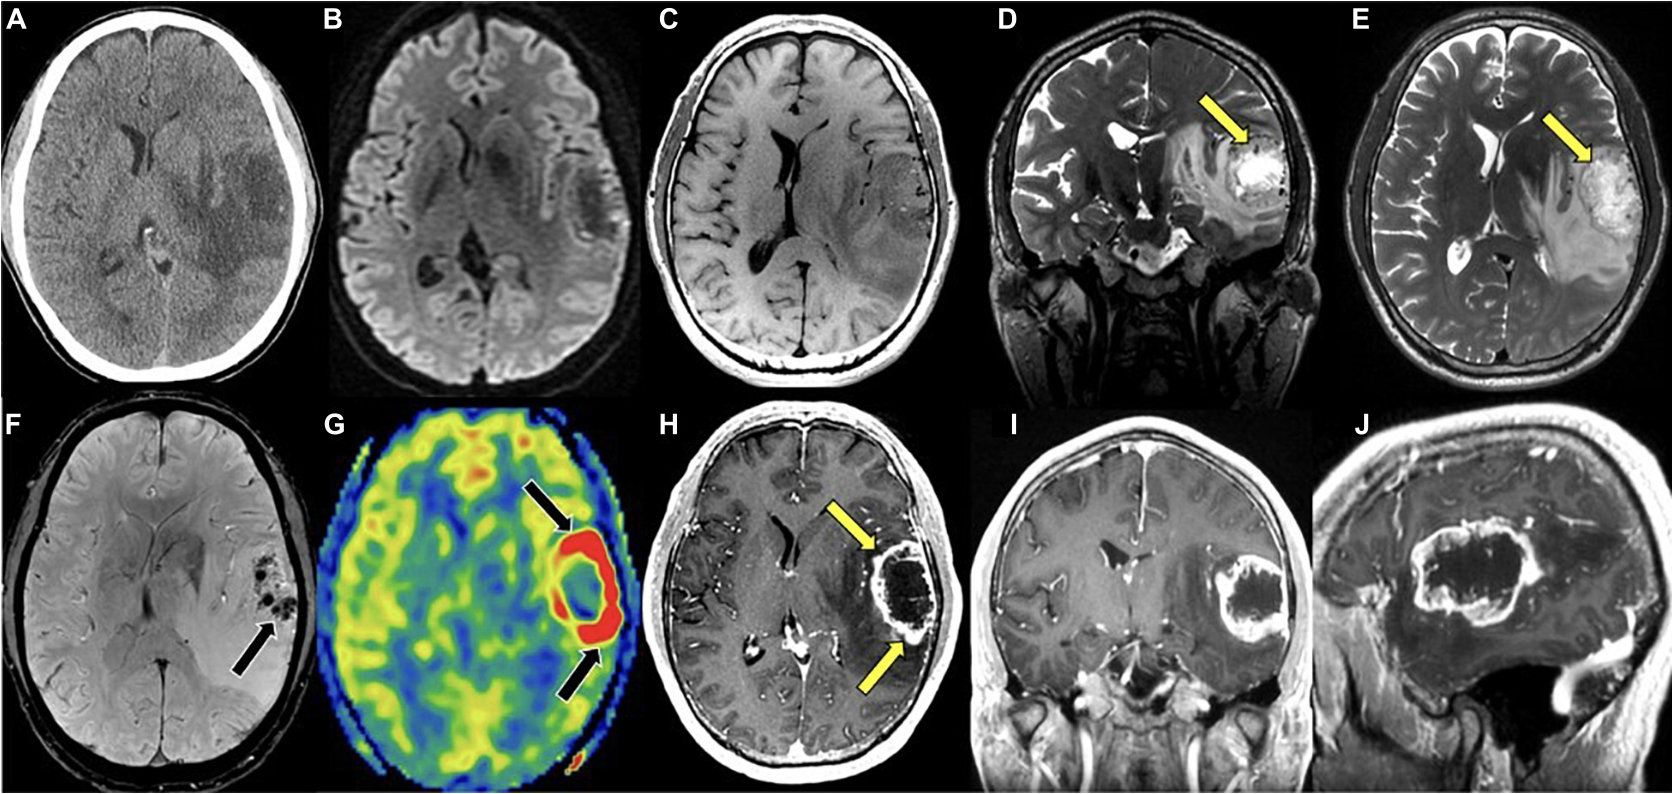
\includegraphics[width=0.85\textwidth]{figures/Figure Intro.png}
    \caption{Glioblastoma, IDH-wildtype multi parametric imaging characteristics. (A) Axial CT without contrast: ill-defined hypodensity lesion centered in the left superior temporal gyrus; (B) axial DWI: no associated reduced diffusion; (C) axial T1 pre contrast: hypointense mass; (D) coronal T2: heterogeneous mass with hypointense rim and prominent central necrosis (yellow arrow); (E) axial T2: heterogeneous mass with hypointense rim and prominent central necrosis (yellow arrow); (F) axial SWI: prominent blood products within the mass (black arrow); (G) axial ASL perfusion: marked hyperperfusion (black arrows) within the rim-enhancing component of the mass; (H) axial T1 post contrast: heterogeneous mass with thick rim enhancement (yellow arrows) and prominent central necrosis; (I) coronal T1 post contrast: heterogeneous mass with thick rim enhancement and prominent central necrosis; (J) sagittal T1 post contrast: heterogeneous mass with thick rim enhancement and prominent central necrosis. Abbreviations: CT, computed tomography; DWI, diffusion weighted imaging; SWI, susceptibility weighted imaging; ASL, arterial spin labeling; MRS, magnetic resonance spectroscopy. Adapted from \cite{carrete2022advanced}}.
    \label{fig:Glioblastoma_multimodal_imaging}
\end{figure}

Magnetic Resonance Imaging(MRI) is the base to every stage of GBM management including diagnosis, surgical 
planing, radiotherapy targeting, treatment response assessment and surveillance for recurrence. Multiparametric 
MRI particularly T1 Weighted(T1W) imaging before and after Gadolinium contrast administratiion, T2 Weighted(T2W) 
imaging and T2 Fluid Attenuated Inversion Recovery(T2-FLAIR) allows clinicians to visualize different tumor 
related compartments. In clinical practice segmentations and radiological assessments commonly distinguish by\cite{almeida2017advanced,FalkDelgado2025}:

\begin{itemize}
    \item \textbf{Necrotic core:} non enhancing central necrosis
    \item \textbf{Enhancing tumor:} contrast enhancing region suggestive of blood brain barrier disruption and active tumor related enhancement
    \item \textbf{Edema/infiltration:} T2-FLAIR hyperintensity that may represent vasogenic edema, infiltrative tumor, or both
    \item \textbf{Resection cavity:} the post surgical cavity and surrounding treatment related changes
\end{itemize}

Longitudinal MRI is specially important after the treatments because changes over time can provide more informative evidence than a single scan. An increase in enhancing volume, new enhancement or increasing T2-FLAIR abnormality may suggest progression but it may also reflect treatment related inflammation, ischemia or radiation injury. Therefore the clinical interpretation of MRI is inherently longitudinal. The same finding can have different implications depending on its timing relative to surgery, Radiotherapy, Chemotherapy and prior imaging.\cite{ellingson2017pseudoprogression}

\subsection{The Pseudoprogression problem}

So after the treatments, serial MRI is used as the principal tool for assessing tumor control, progression and the treatment related injury. However conventional MRI cannot always distinguish true tumor progression from the pseudoprogression or radiation necrosis. Because all of these changes can produce contrast enhancement or T2/FLAIR signal variations.\cite{barajas2019pseudoprogression}. Further more, Pseudoprogression refers to a new enlarging area of contrast enhancement that occurs in the absence of true tumor growth and subsequently stabilize or resolves without a change in therapy. It is thought to reflect treatment induced inflammatory changes, vascular permeability and blood brain barrier disruption rather than proliferating tumor. Radiation necrosis is related but typically later occurring treatment effect can also mimic recurrent tumor on conventional MRI. This distraction is difficult because of pseudoprogression. Radiation necrosis and true progression can all increaing contrast enhancement, mass effect, peritumoral edema and worsening the neurological symptoms.\cite{thust2018pseudoprogression}.

\begin{figure}[htbp]
    \centering
    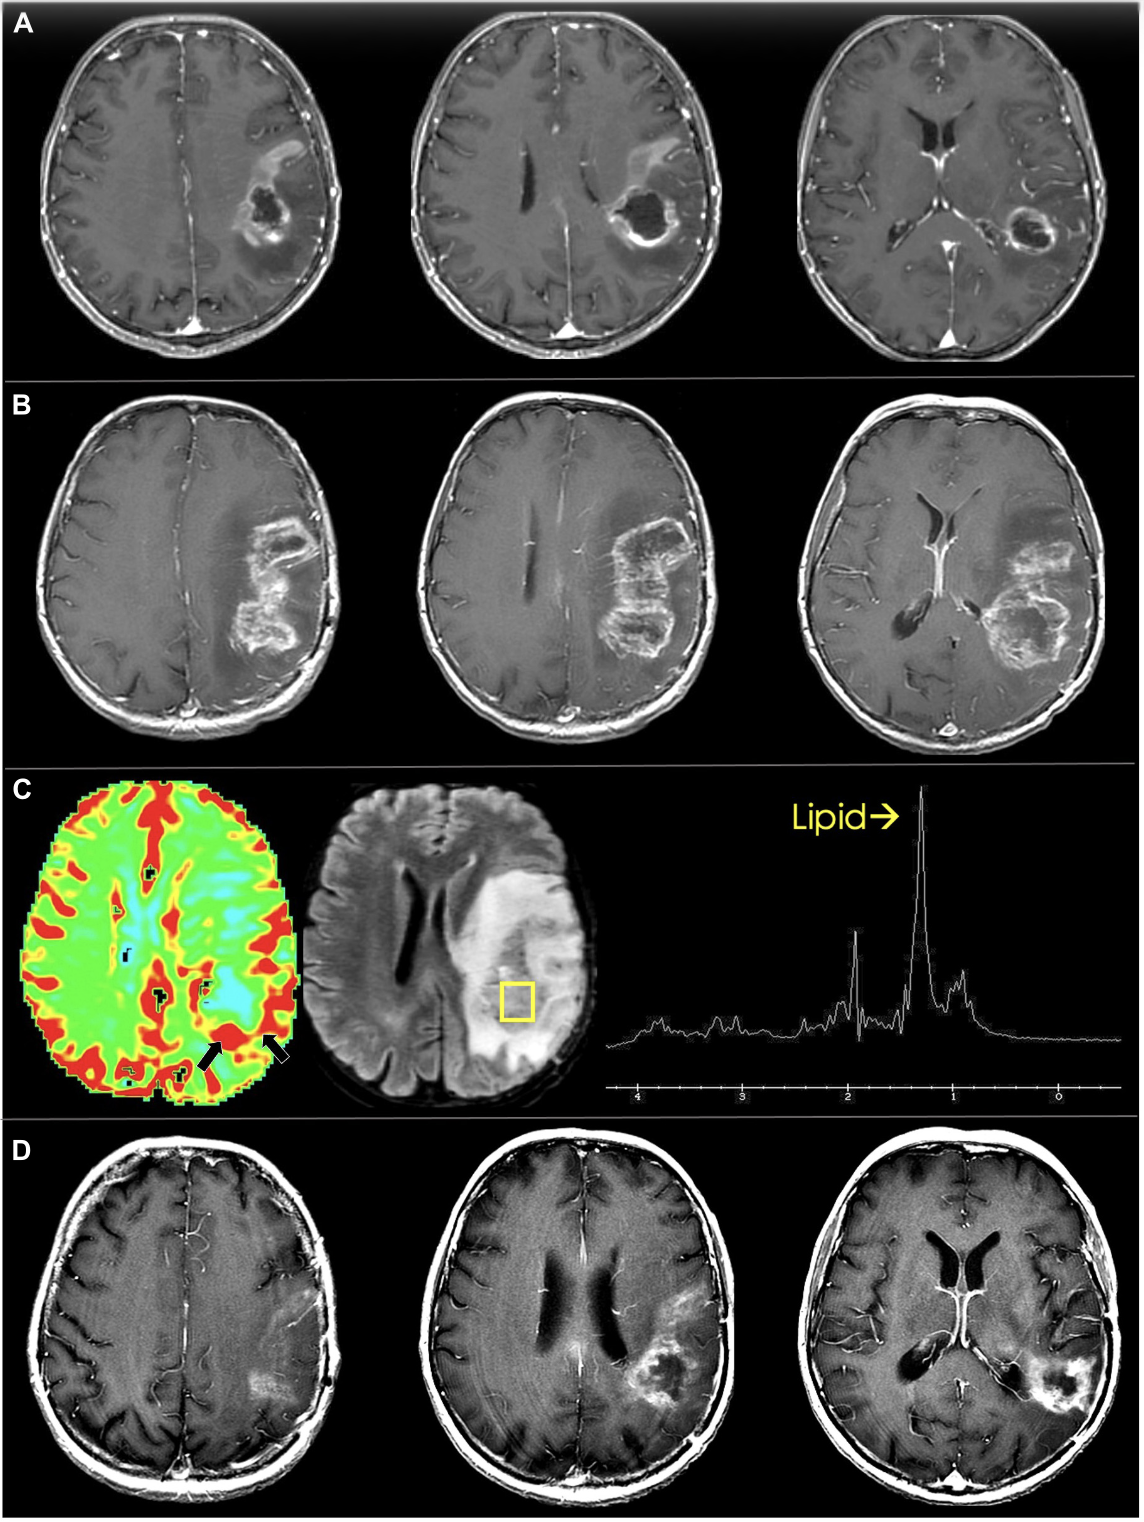
\includegraphics[width=0.85\textwidth]{figures/Figure Pseudoprogression.png}
    \caption{Pseudoprogression in Glioblastoma. (A) Immediate pre Radiotherapy: axial T1 post contrast images show rim enhancing and centrally necrotic left frontoparietal Glioblastoma; (B) Eight week follow-up: immediate post Radiotherapy axial T1 post contrast images show marked increase in enhancement and necrosis; (C) dynamic susceptibility weighted contrast enhanced perfusion MRI shows mild increase in blood volume along the posterior rim (black arrows), while single voxel proton spectroscopy targeted to the posterior component shows a markedly increased lipid peak suggesting tissue necrosis; (D) Three month follow up: axial T1 contrast images show marked decrease in enhancement and necrosis of the treated Glioblastoma. Adapted from \cite{carrete2022advanced}.}
    \label{fig:glioblastoma_pseudoprogression}
\end{figure}

This doubtfulness is clinically consequential. A patient with pseudoprogression may be incorrectly considered to have progressive disease, whereas a patient with true progression may experience delayed escalation of therapy. Current reviews emphasize that conventional MRI alone is often insufficient and histopathology remains the reference standard in ambiguous cases.\cite{tran2013treatment}. The clinical consequences of this uncertainty are substantial:

\begin{itemize}
    \item A patient with pseudoprogression may be incorrectly classified as having progressive disease, potentially leading to premature discontinuation of effective therapy or unnecessary escalation.
    \item A patient with true progression may have treatment escalation delayed while awaiting confirmatory imaging.
    \item Repeated imaging, advanced MRI, positron emission tomography, or tissue sampling may be required, increasing cost, delay, patient burden, and diagnostic uncertainty.
\end{itemize}

Advanced imaging techniques including perfusion MRI, Diffusion Weighted Imaging, Magnetic Resonance Spectroscopy and Amino Acid \texttt{PET} can provide additional information. However even these modalities do not always provide a definitive distinction between pseudoprogression and true progression.\cite{delgado2018treatment}.

\subsection{The need for the longitudinal interpretation}

Current response assessment frameworks including the Response Assessment in Neuro Oncology(RANO) criteria recognize that interpretation must account the treatment time. RANO 2.0 specially highlights the pseudoprogression is frequent during the first 12 weeks after the Radiotherapy. During this period, progression generally requires confirmation by repeat MRI or histopathological evidences of recurrent tumor. Therefore a Digital Twin (DT) should not simply interpret an increase in enhancing volume as progression. It should incorporate scan timing, treatment exposure, molecular context and longitudinal trajectory.\cite{wen2023rano20}.

\begin{figure}[htbp]
    \centering
    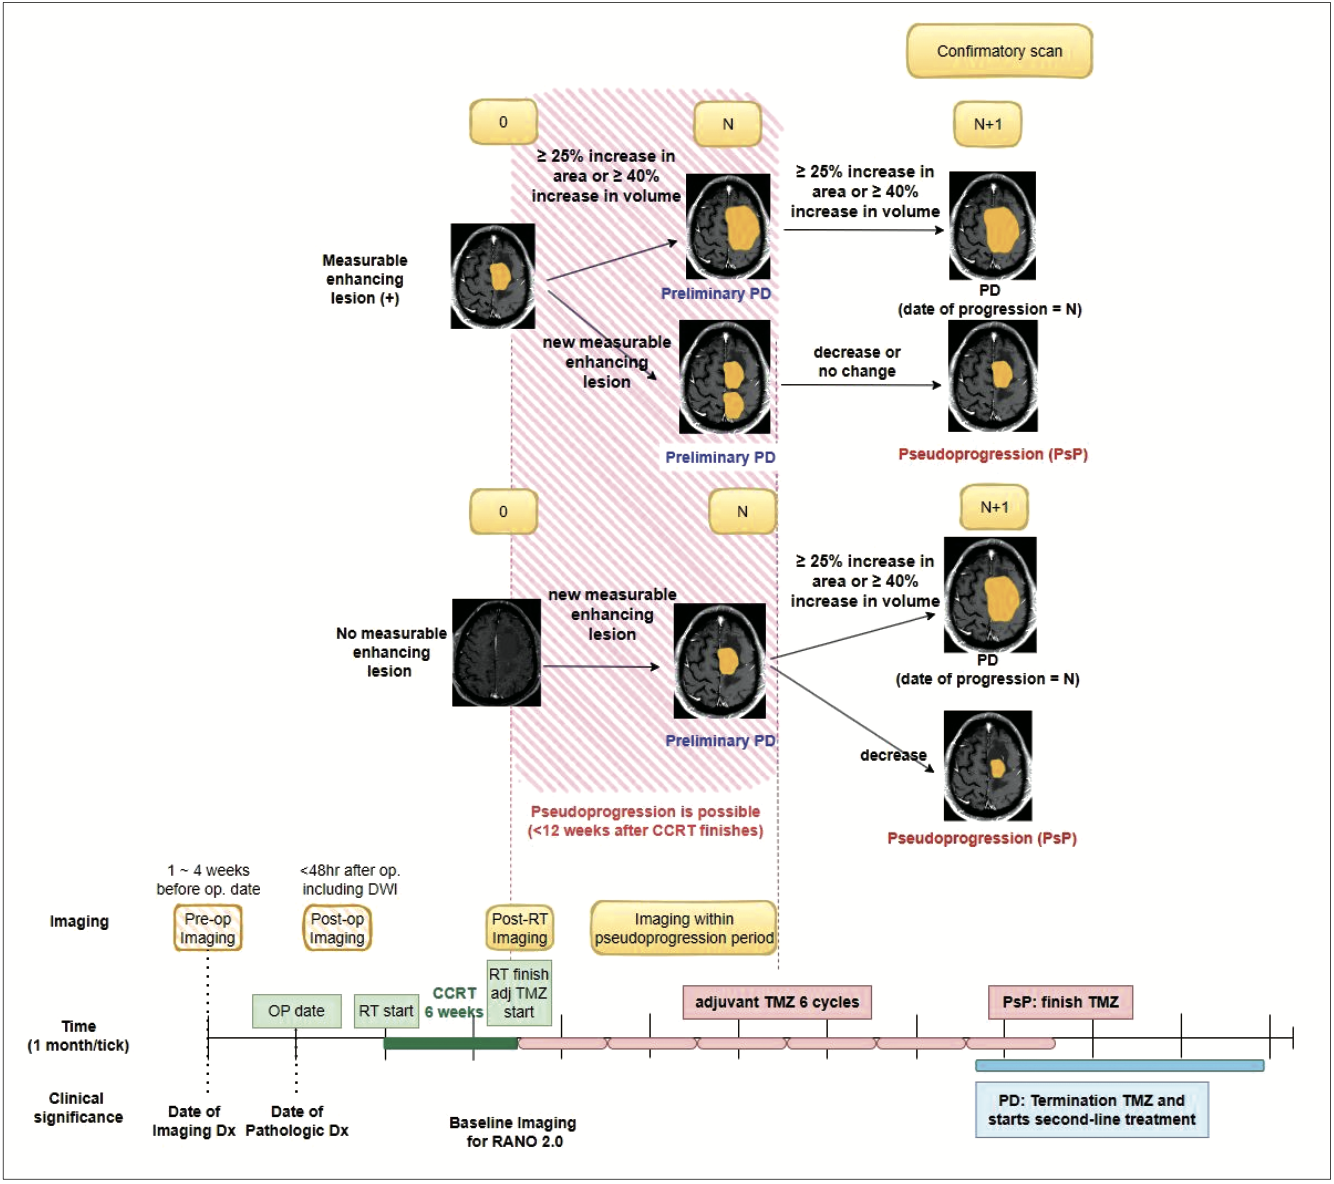
\includegraphics[width=1.00\textwidth]{figures/Figure RANO.png}
    \caption{Longitudinal response assessment according to the Response Assessment in 
    Neuro-Oncology (RANO) 2.0 criteria. In newly diagnosed Glioblastoma, the post Radiotherapy 
    MRI is used as the baseline for subsequent response assessment. Because pseudoprogression 
    is frequent during the first 12 weeks after completion of radiotherapy or concurrent 
    chemoradiotherapy, apparent progression during this period requires confirmation by repeat 
    MRI or histopathological evidence of unequivocal recurrent tumor before progressive disease 
    is declared. This temporal framework highlights the importance of incorporating scan timing, 
    treatment exposure, and serial imaging trajectories into computational models of tumor 
    dynamics. Adapted from \cite{sakata2024rano}.}
    \label{fig:rano2_pseudoprogression_timeline}
\end{figure}

This has two important implications for computational modeling. First a model that interprets an increase in enhancing tumor volume as tumor growth without considering the time since, Radiotherapy may misclassify treatment related inflammation as progress. Early post treatment enhancing expansion should therefore be interpreted in the context of Radiotherapy completion date, Chemotherapy exposure steroid use and subsequent imaging trajectory. Secondly a single MRI timepoint provides limited information about tumor dynamics. The rate of change in tumor volume, enhancing tissue, edema and imaging heterogeneity may be more informative than any individual measurement. Longitudinal features such as volume velocity, voxel count velocity, intensity change and heterogenity change can capture temporal behavior that is invisible in a static scan. \cite{sakata2025rano}.

\subsection{Molecular heterogeneity and personalized care}

\begin{figure}[htbp]
    \centering
    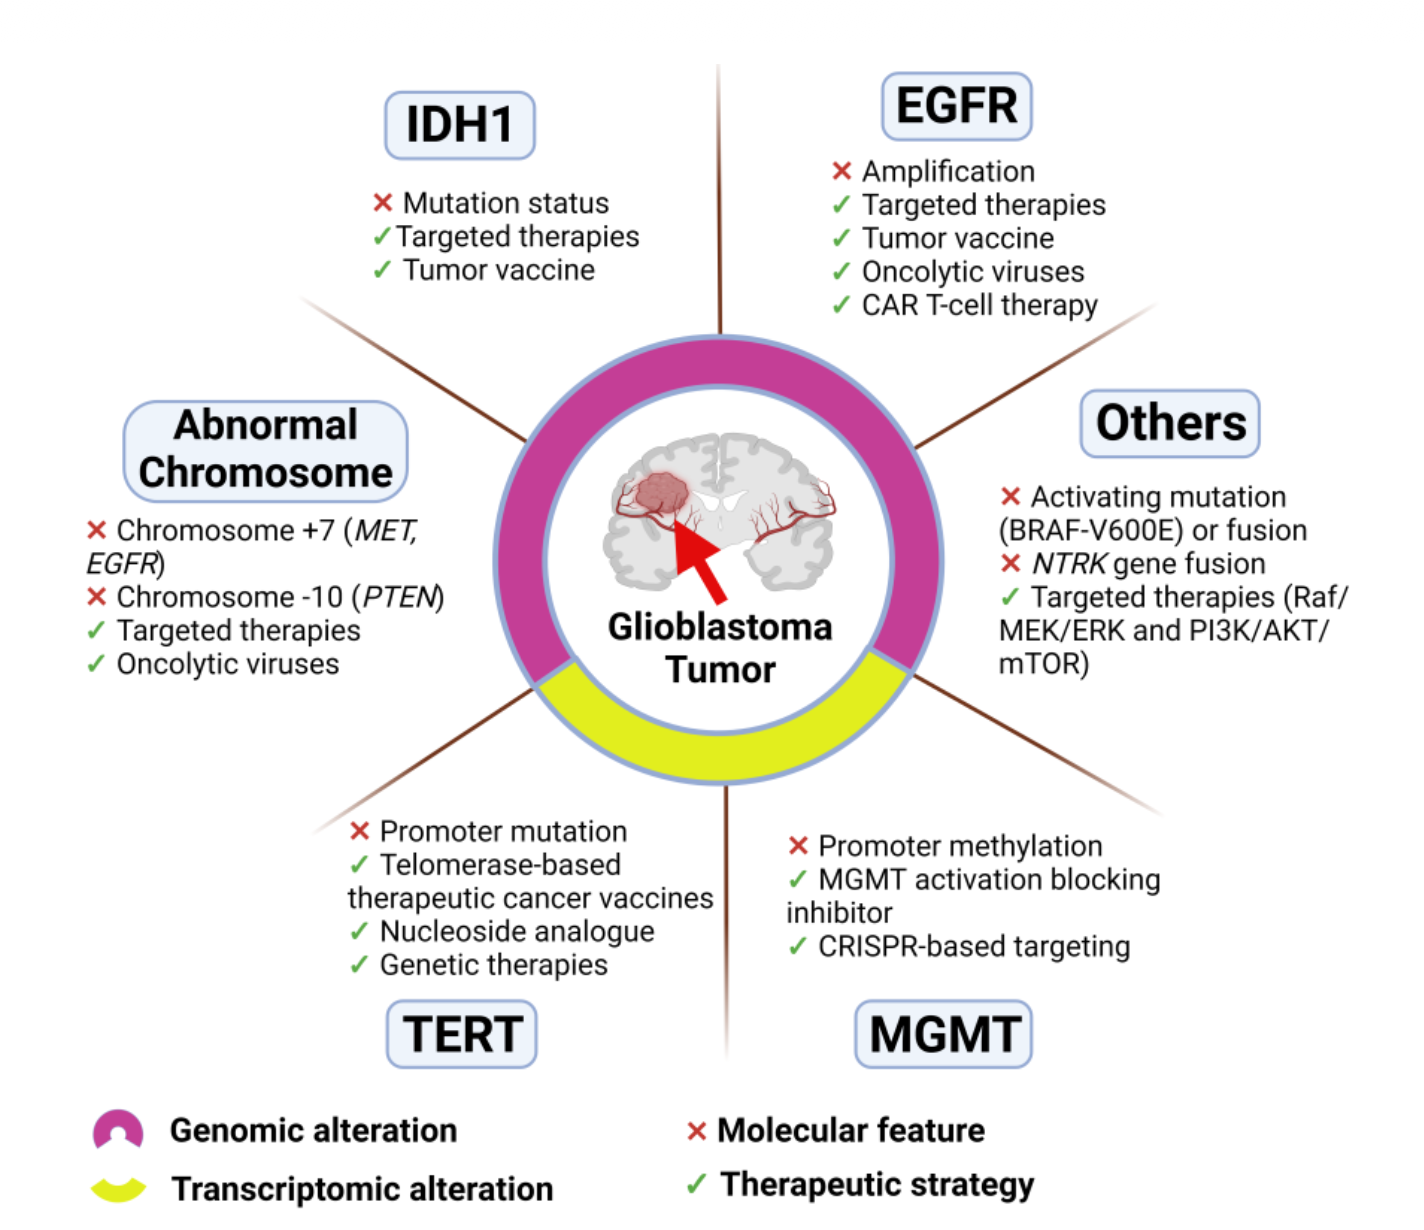
\includegraphics[width=0.85\textwidth]{figures/Figure Molecular Hetoregeneity.png}
    \caption{Molecular heterogeneity in Glioblastoma. Molecular alterations, including \textit{IDH} mutation status, \textit{MGMT} promoter Methylation, \textit{TERT} promoter mutation, \textit{EGFR} amplification, \textit{PTEN} alteration, \textit{CDKN2A/B} deletion, and \textit{TP53} alteration, influence prognosis, treatment sensitivity, and expected tumor behavior. \textit{IDH}-mutant Gliomas generally have a more favorable prognosis than \textit{IDH}-wildtype tumors, whereas \textit{MGMT} promoter methylation is associated with greater temozolomide sensitivity and improved survival. These molecular features provide important biological context for interpreting apparently similar MRI phenotypes and for personalizing computational models of tumor growth and treatment response. Adapted from \cite{zhu2024molecular}.}
    \label{fig:gbm_molecular_heterogeneity}
\end{figure}

Glioblastoma is not a biologically uniform disease. Molecular features strongly influence prognosis, treatment sensitivity, and expected tumor behavior. Molecular markers such as \texttt{IDH} mutation, \texttt{MGMT} promoter Methylation, \texttt{1p/19q} codeletion, \texttt{TERT }promoter mutation, \texttt{EGFR} amplification, \texttt{PTEN} alteration, \texttt{CDKN2A/B} deletion, and \texttt{TP53} alteration are established prognostic and predictive factors. Meta analytic evidence support their positive prognostic significance across treatment types.\cite{karsy2015practical}. 

\texttt{IDH} mutant Glioma generally have a more favorable prognosis than \texttt{IDH} wildtype tumors, whereas \texttt{IDH} wildtype GBM tends to behave more aggressively. \texttt{MGMT} promoter methylation is both prognostic and predictive. MGMT methylation was significantly associated with better overall survival, with a pooled hazard ratio of 1.66 for unmethylated versus methylated status.\cite{noroxe2016hallmarks}. Also \texttt{MGMT} promoter Methylation is associated with greater sensitivity to Temozolomide and longer survival. In \texttt{IDH} wildtype Glioblastoma, methylated \texttt{MGMT} has been associated with a median overall survival of approximately 24 months, compared with approximately 14 months in unmethylated tumors.\cite{melhem2022updates}.

These variables should therefore not be treated as optional metadata. They provide biological context that may help to explain why two patients with similar MRI appearances can have very different growth rates, treatment responses and survival outcome.

\subsection{Limitations of current decision support and Digital twins as a potential solution}

At present clinical decision making commonly relies on visual interpretation of serial MRI, volumetric or bidimensional RANO measurements, clinical symptoms and corticosteroid use, molecular markers and multidisciplinary tumor board discussions. These sources of information are essential but they are often assessed separately. Imaging findings may not be explicitly linked to the patients treatment timeline, molecular profile and longitudinal outcome trajectory. Furthermore conventional assessments provides limited formal quantification of uncertainty. Clinicians may recognize that a finding of uncertain but they rarely receive a calibrated estimate of probability that a given trajectory represents progression versus treatment effect. This creates a need for a framework that can integrate heterogeneous patient specific data into a coherent, quantitative representation of tumor behavior\cite{luemerson2026corticosteroids}.

A Digital Twin(DT) is a patient specific computational representation that integrates clinical, imaging, molecular and treatment data to simulate disease behavior and support decision making. In oncology Digital Twin(DT)s can combine observed patient data with mechanistic models to estimate hidden biological processes, forecast future disease trajectory and quantify uncertainty. For Glioblastoma, a digital twin could integrate:

\begin{itemize}
    \item Serial MRI derived tumor volumes
    \item Tumor compartment segmentations
    \item Intensity and heterogeneity features
    \item Molecular biomarkers
    \item Treatment timing and exposure
    \item Clinical outcomes such as progression free survival and overall survival
\end{itemize}

Reaction diffusion models are particularly suitable for this purpose because they represent two central processes of Glioblastoma biology. Local proliferation and diffusion driven invasion into surrounding brain tissue. When personalized with imaging data, these models can estimate tumor dynamics beyond the visible enhancing margin and may predict infiltrative growth not directly captured by MRI.


\begin{equation}
    \frac{\partial N(x,t)}{\partial t} = D \nabla^2 N(x,t) + \rho N(x,t)\left(1 - \frac{N(x,t)}{K}\right) - R(N,t),
    \label{eq:fisher_kpp_custom}
\end{equation}

Fisher–KPP reaction diffusion model provides a compact mathematical representation of these processes. where $N(x,t)$ is the tumor cell density, while $D$ represents the invasion/diffusion, $\rho$ represents proliferation, then $K$ is the carrying capacity, and $R(N,t)$ represents the treatment induced cell kill or growth inhibition. \cite{fritz2025timefractional}.

By calibrating such a model to a patient specific serial MRI derived tumor volumes helps to estimate parameters such as rate of proliferation and spacial invasion, that are not directly observable from a single scan. This patient specific reaction diffusion approaches including physics informed neural network(PINN) methods have been developed to infer Glioblastoma infiltration parameters from structural MRI.

\subsection{Clinical value of the proposed Digital Twin}

A patient linked Digital Twin could support clinical decision making in several ways:

\begin{itemize}
    \item \textbf{Earlier risk stratification:} identify patients whose estimated proliferation or invasion rates suggest higher risk of progression.
    \item \textbf{Longitudinal interpretation:} place a new MRI finding in the context of the patient's prior trajectory and treatment timeline.
    \item \textbf{Pseudoprogression-aware monitoring:} avoid overinterpreting early post-radiotherapy enhancement by incorporating time since treatment and subsequent imaging evolution.
    \item \textbf{Personalized forecasting:} estimate future tumor burden with uncertainty intervals rather than providing a single deterministic prediction.
    \item \textbf{Treatment-scenario exploration:} simulate how alternative treatment assumptions might affect predicted tumor dynamics.
    \item \textbf{Decision support:} provide clinicians with an additional quantitative tool alongside RANO assessment, clinical examination, and multidisciplinary review.
\end{itemize}

The objective is not to replace clinical judgement or RANO criteria. The Digital Twin would complement RANO assessment, clinical examination, molecular diagnostic and multidisciplinary review by providing a quantitative  patient specific and uncertainty aware representation of tumor behavior.

\subsection{Research Motivation}

Despite growing interest in Digital twin for neuro oncology, major challenges remain. Many existing models are developed using single snapshot imaging data, do not incorporate treatment timing, or do not explicitly link model derived tumor dynamics to longitudinal clinical outcomes. In addition, imaging, molecular, treatment and survival data re often stored in separated formats and analyzed independently and limiting their usefulness for patient specific modeling.

This project addresses these limitations by developing a patient linked Digital Twin framework for Glioblastoma. The framework integrates longitudinal MRI derived tumor measurements, Radiomic descriptors, molecular priors, treatment exposure and survival outcomes with a unified computational pipeline. By calibrating a Fisher KPP based tumor growth model to patient specific longitudinal data the proposed Digital Twin aims to estimate individual tumor dynamics, forecast future tumor burden with uncertainty and explore associations between model derived dynamics and clinical outcomes.

Ultimately the goal is to move beyond static population level prediction toward a reproducible patient specific framework that can support more informed and personalized decision making in Glioblastoma care.

